\section{Frequency mode 02}
\label{sec:fm02}

\subsection{Overview}
\label{sec:fm02:overview}
Frequency mode~02 monitors the band $544.102$--$544.902\,\mathrm{GHz}$. Its
main use is retrievals of \chem{O_3} and \chem{HNO_3}.  This mode was intended to be the main measurement of ozone in the stratosphere but in previous versions of the data products suffered with large systematic biases.  We believe that this was caused by an incorrect line broadening constant. This also resulted in an unrealistic pointing offset being derived for this band.  In this version of the product the coefficient was adjusted to remove the pointing offset and at the same time greatly improved the ozone values. 
 

\TODO{Show spectra?}

\subsection{Comparison of retrieved profiles}
\label{sec:fm02:comparison}


%%%%%%
% O3 %
%%%%%%

\subsubsection{\chem{O_3}}
\label{sec:fm02:comparison:O3}
The retrievals for \chem{O_3} have been compared with data from the MIPAS, MLS,
OSIRIS and SAGE~III instruments. Annual average differences to these
instruments are shown in Figure~\ref{fig:fm02:O3:profiles}. In
Figure~\ref{fig:fm02:O3:scatter} individual retrievals for the instruments for
the entire period are plotted against the retrievals from the new and old
versions of the \smr\ processing chain. The results show a considerable
improvement with the updated version of the processing, with much better
over-all correlation and coherency, and most of the systematic under
estimation having been removed compared to all the considered instruments. The
largest improvement is compared to SAGE~III, though, as seen in
Figure~\ref{fig:fm02:O3:profiles:SAGEIII}, there are still large systematic
differences depending on the altitude.  This could be a result of the difference in local time at the measurement location. At these altitudes ozone starts to exhibit a dirunal variation. This speculation could be supported by the good agreement with SAGE since it is a occultation instrument it measures closest to Odin's local time.  Figure~\ref{fig:fm02:O3:mr_avk} suggests that the product is useful over the range 10-20 km with a vertical resolution of around 3 km. 


\begin{figure}[htpb]
    \centering
    \begin{subfigure}[b]{0.49\textwidth}
        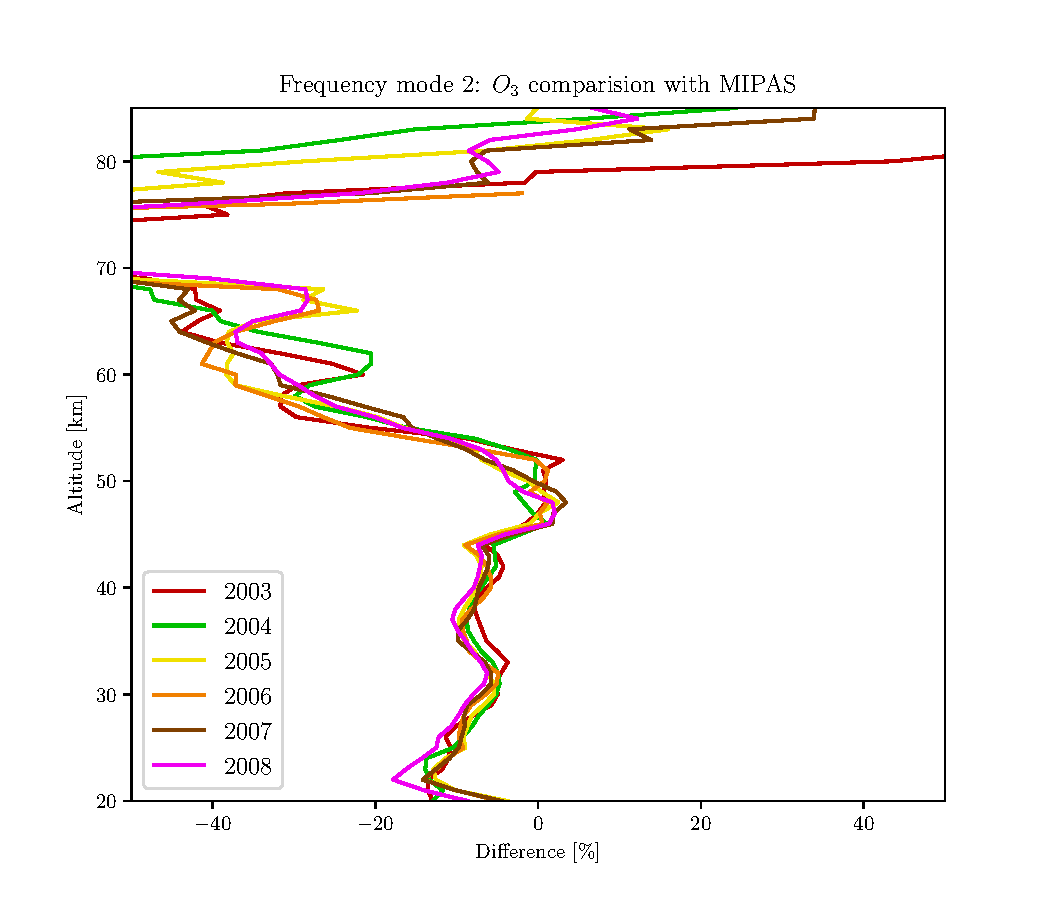
\includegraphics[width=\textwidth]{DDS_fm2_O3_perdiff_mipas}
        \caption{average difference to MIPAS}
        \label{fig:fm02:O3:profiles:MIPAS}
    \end{subfigure}
    \,
    \begin{subfigure}[b]{0.49\textwidth}
        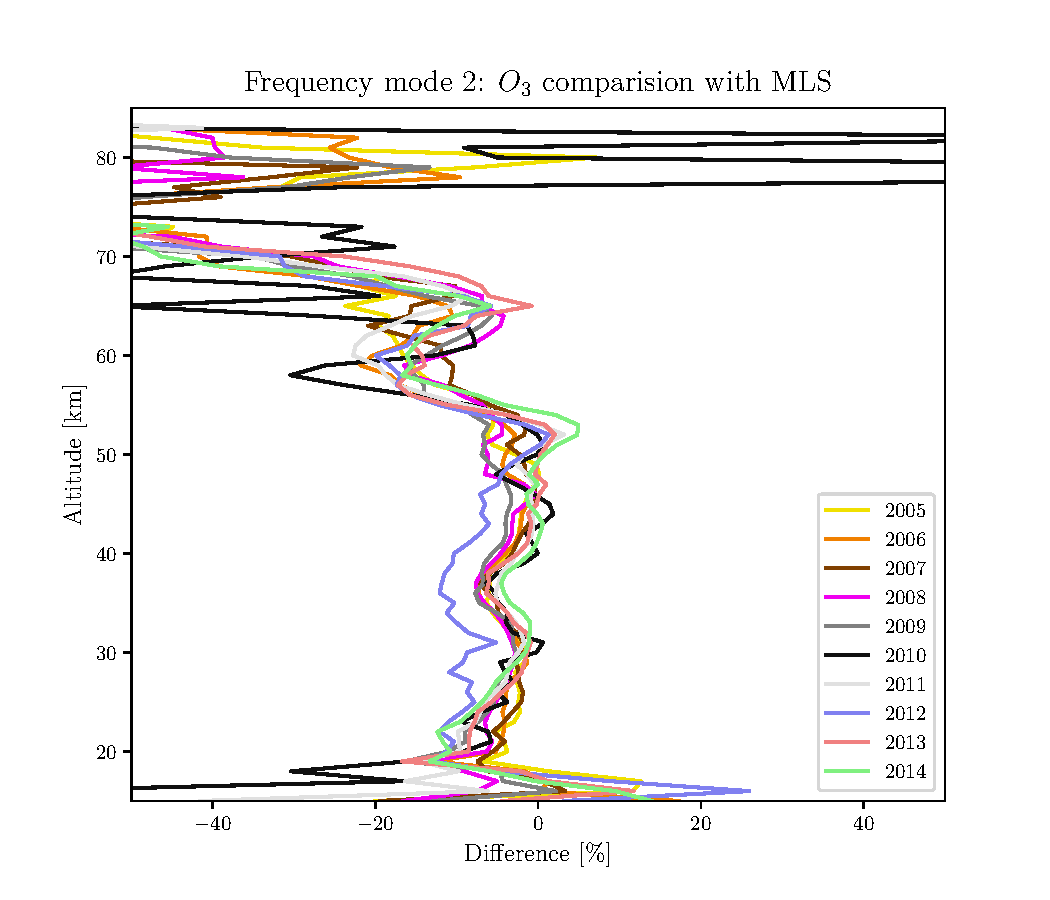
\includegraphics[width=\textwidth]{DDS_fm2_O3_perdiff_mls}
        \caption{average difference to MLS}
        \label{fig:fm02:O3:profiles:MLS}
    \end{subfigure}

    \begin{subfigure}[b]{0.49\textwidth}
        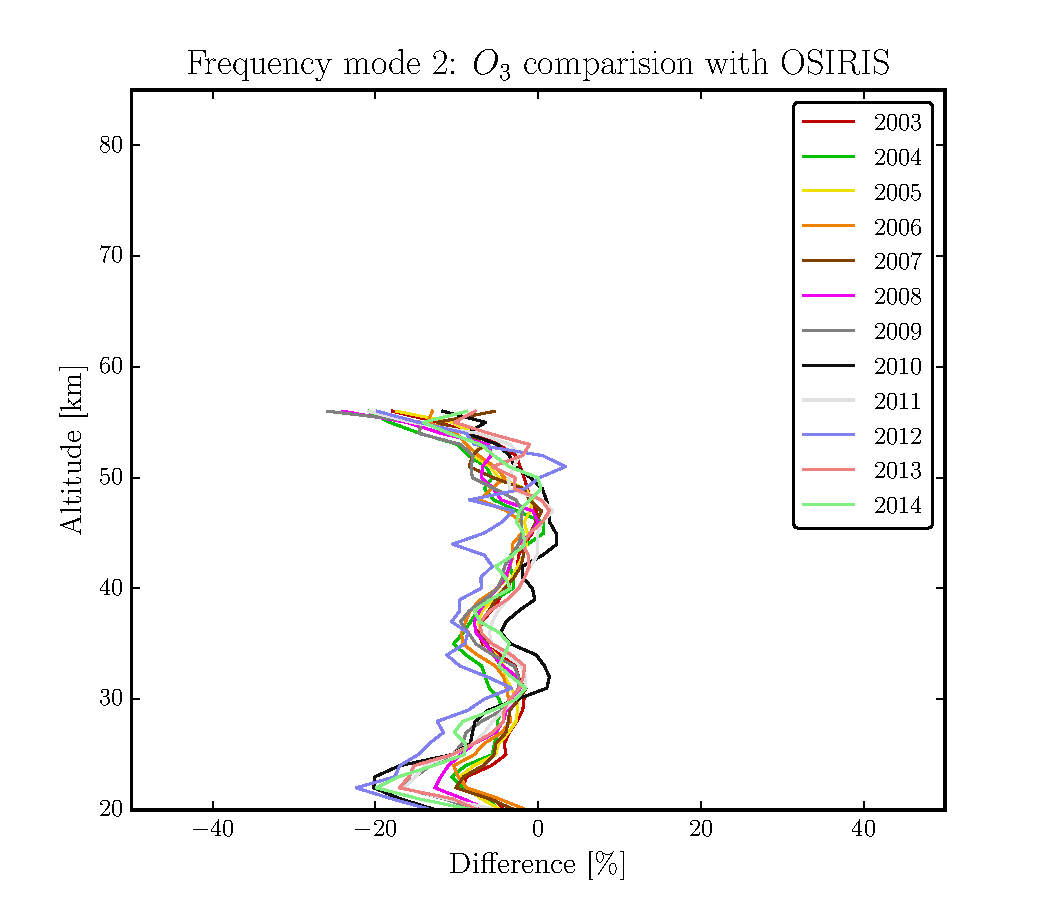
\includegraphics[width=\textwidth]{DDS_fm2_O3_perdiff_osiris}
        \caption{average difference to OSIRIS}
        \label{fig:fm02:O3:profiles:OSIRIS}
    \end{subfigure}
    \,
    \begin{subfigure}[b]{0.49\textwidth}
        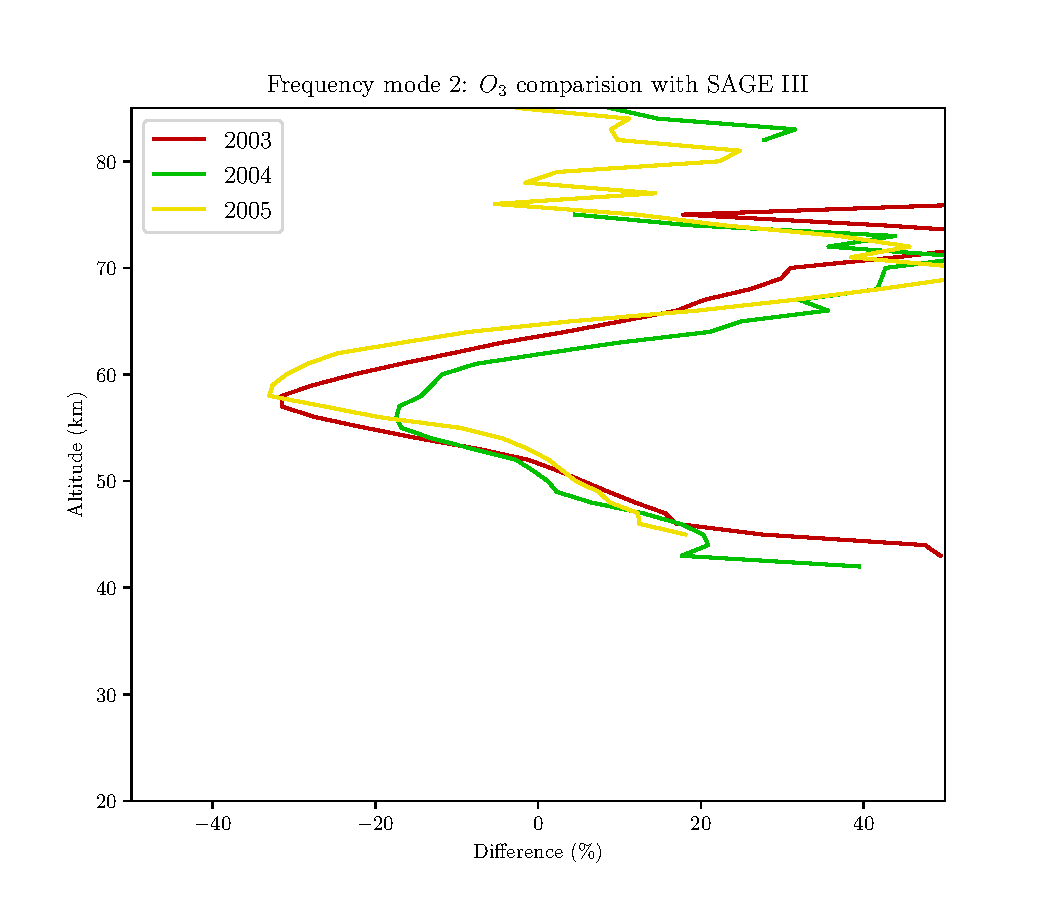
\includegraphics[width=\textwidth]{DDS_fm2_O3_perdiff_sage}
        \caption{average difference to SAGE~III}
        \label{fig:fm02:O3:profiles:SAGEIII}
    \end{subfigure}
    \caption{Average difference in percent between retrievals of \chem{O_3}
    from \smr~v3 and collocated measurements from various instruments at
    different altitudes for frequency mode~02. (Retrievals yielding
    concentrations $\leq 0.1\,\mathrm{ppm}$ have been filtered out.)}

    \label{fig:fm02:O3:profiles}
\end{figure}

\begin{figure}[htpb]
    \centering
    \begin{subfigure}[b]{0.49\textwidth}
        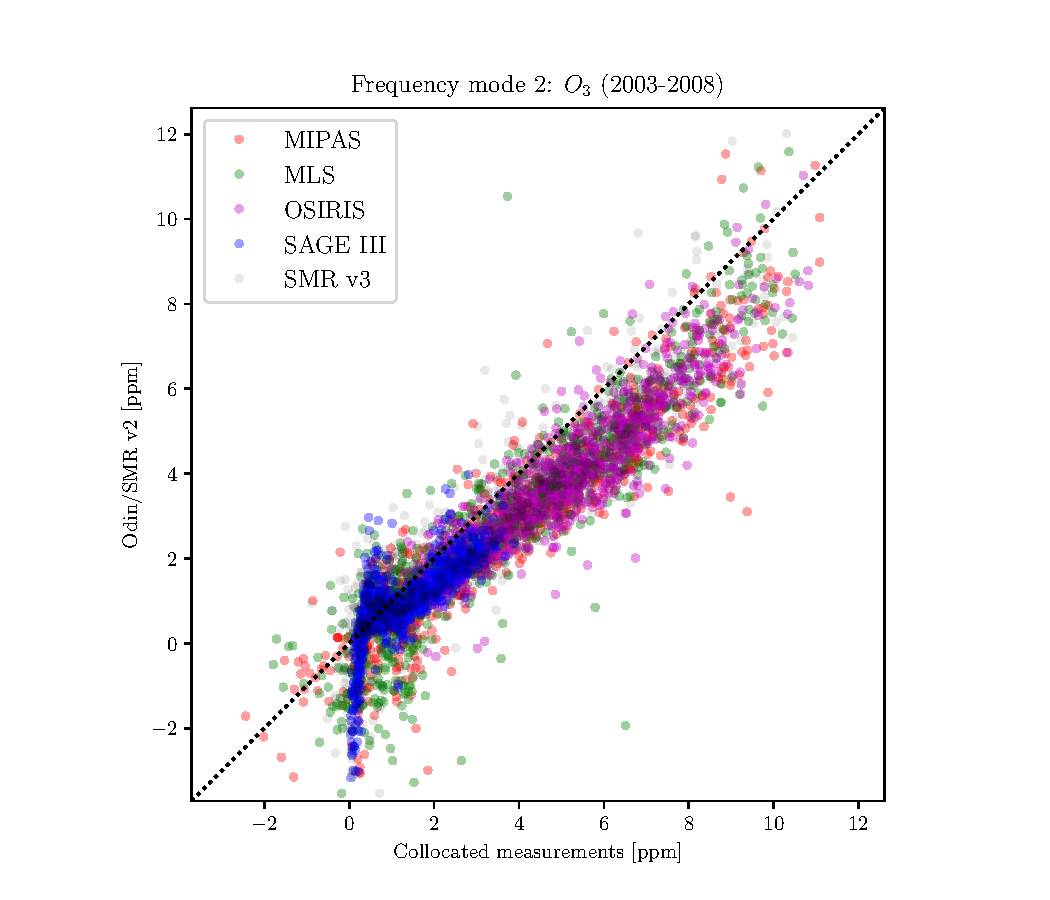
\includegraphics[width=\textwidth]{DDS_fm2_O3_scatter_v2}
        \caption{correlation of collcated instruments with \smr~v2.X}
        \label{fig:fm02:O3:scatter:v2}
    \end{subfigure}
    \,
    \begin{subfigure}[b]{0.49\textwidth}
        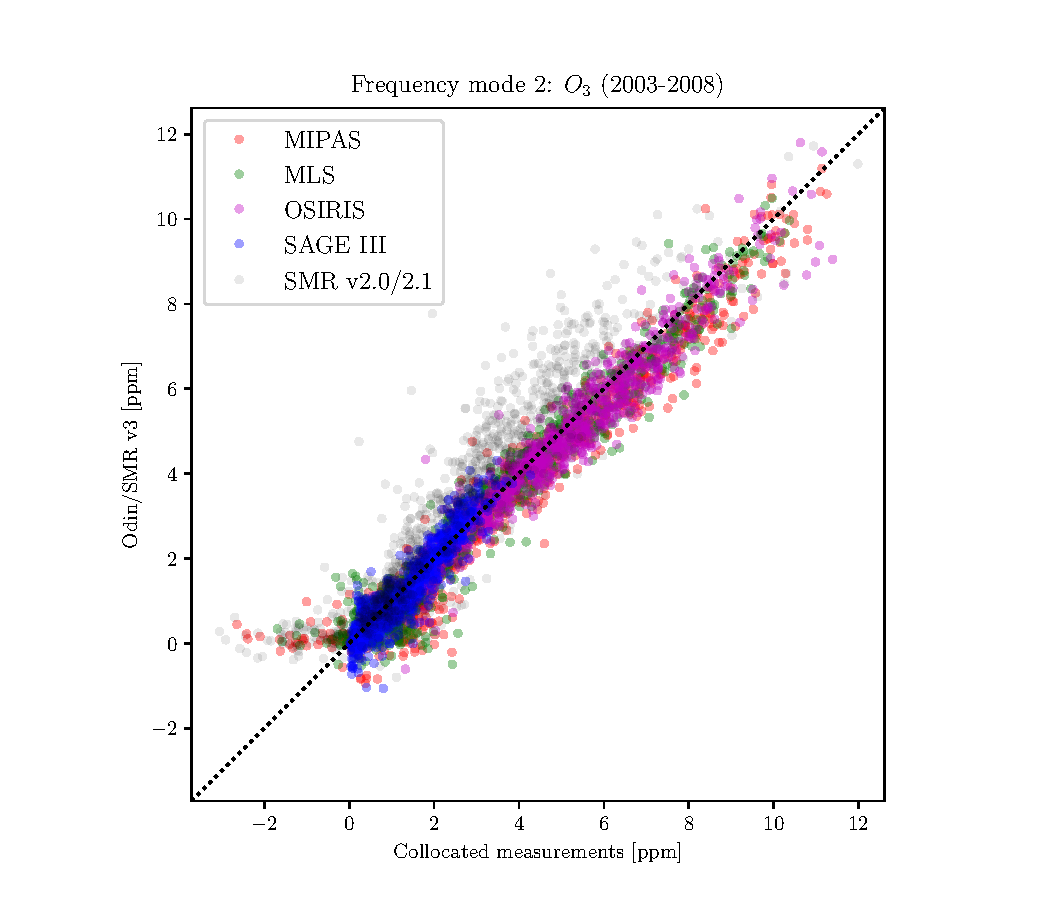
\includegraphics[width=\textwidth]{DDS_fm2_O3_scatter_v3}
        \caption{correlation of collcated instruments with \smr~v3}
        \label{fig:fm02:O3:scatter:v3}
    \end{subfigure}
    \caption{Correlation between retrievals of \chem{O_3} using \smr\
    versions~2.X and~3 and collocated measurements from various instruments
    for frequency mode~02.}
    \label{fig:fm02:O3:scatter}
\end{figure}

\begin{figure}[htpb]
    \centering
    \begin{subfigure}[b]{0.49\textwidth}
        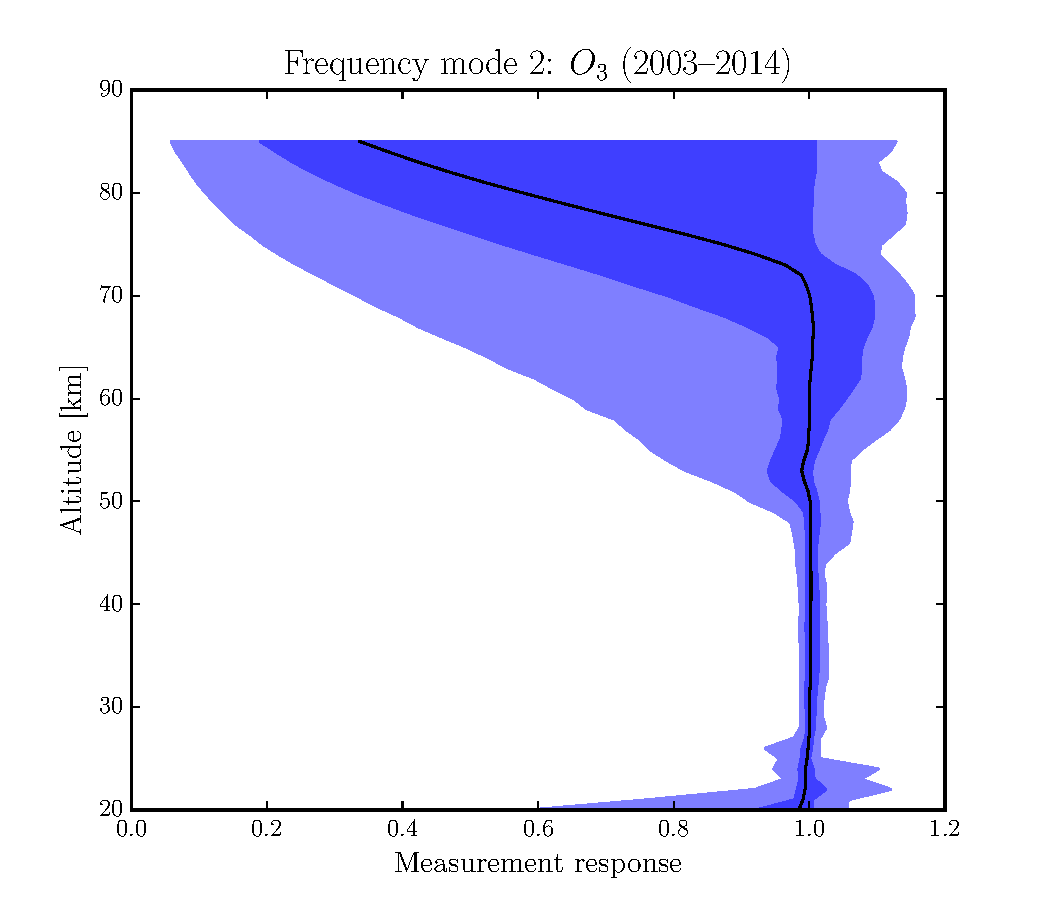
\includegraphics[width=\textwidth]{DDS_fm2_O3_mr}
        \caption{median measurement response with $1\sigma$ and $2\sigma$
        percentiles}
        \label{fig:fm02:O3:mr}
    \end{subfigure}
    \,
    \begin{subfigure}[b]{0.49\textwidth}
        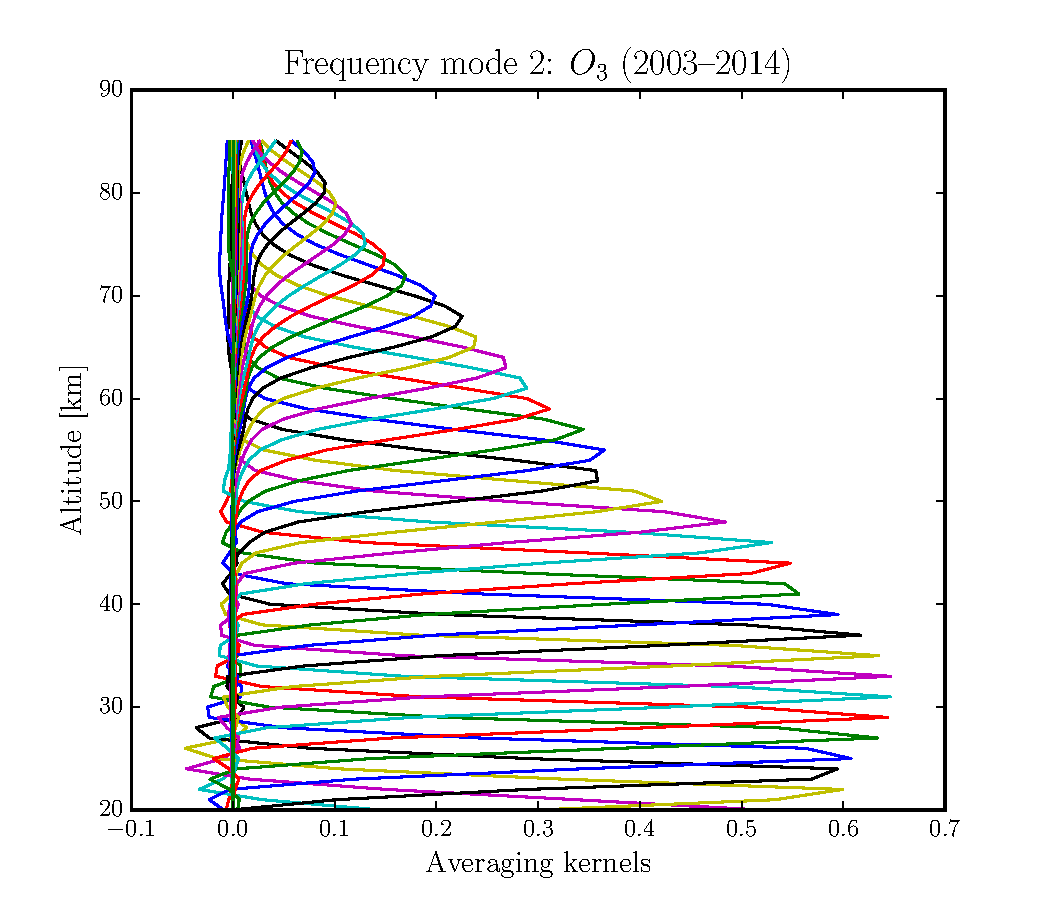
\includegraphics[width=\textwidth]{DDS_fm2_O3_avk}
        \caption{median averaging kernels\newline~}
        \label{fig:fm02:O3:avk}
    \end{subfigure}
    \caption{Measurement response and averaging kernels for \chem{O_3}
    retrievals for \smr~v3 at different altitudes for frequency mode~02.}
    \label{fig:fm02:O3:mr_avk}
\end{figure}


%%%%%%%%
% HNO3 %
%%%%%%%%

\subsubsection{\chem{HNO_3}}
\label{sec:fm02:comparison:HNO3} The retrievals for \chem{HNO_3} have been
compared with data from the MIPAS and MLS instruments. Annual average
differences to these instruments are shown in
Figure~\ref{fig:fm02:HNO3:profiles}. In Figure~\ref{fig:fm02:HNO3:scatter}
individual retrievals for the instruments for the entire period are plotted
against the retrievals from the new and old versions of the \smr\ processing
chain. The results show a considerable improvement with the updated version of
the processing compared to both considered instruments with respect to the over-all
correlation and coherency is much better, However a large
altitude dependent difference seems to have been introduced, resulting in \smr\ over
estimating the concentrations.  The reason for this has not been identified. 
Figure~\ref{fig:fm02:HNO3:mr_avk} suggests that the product is useful over the range 10-50 km with a vertical resolution of around 4 km. 

\begin{figure}[htpb]
    \centering
    \begin{subfigure}[b]{0.49\textwidth}
        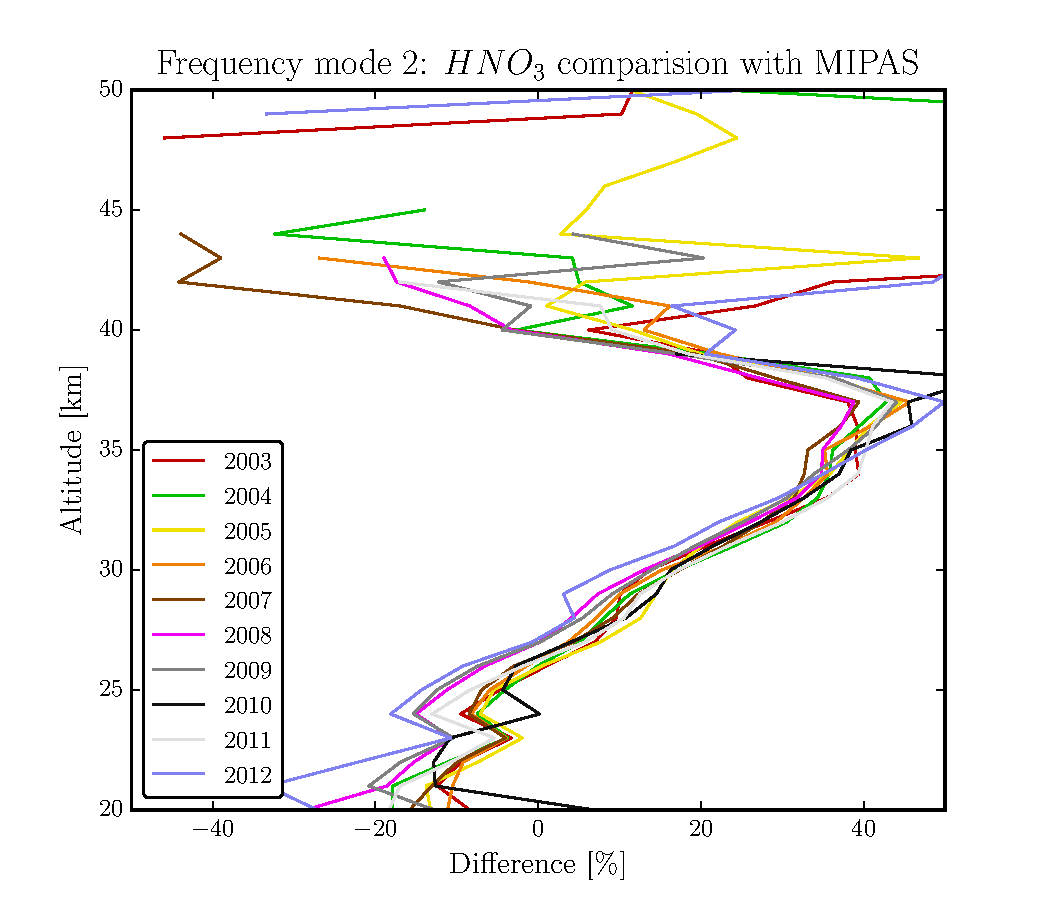
\includegraphics[width=\textwidth]{DDS_fm2_HNO3_perdiff_mipas}
        \caption{average difference to MIPAS}
        \label{fig:fm02:HNO3:profiles:MIPAS}
    \end{subfigure}
    \,
    \begin{subfigure}[b]{0.49\textwidth}
        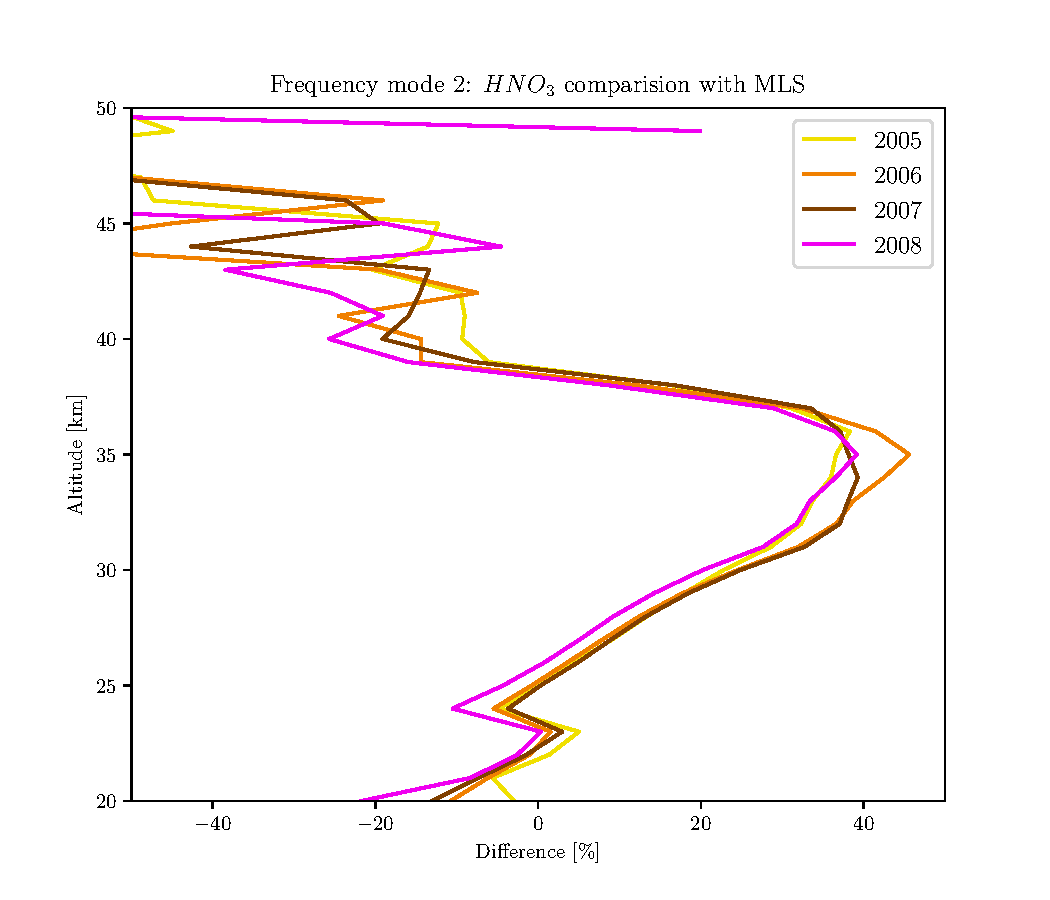
\includegraphics[width=\textwidth]{DDS_fm2_HNO3_perdiff_mls}
        \caption{average difference to MLS}
        \label{fig:fm02:HNO3:profiles:MLS}
    \end{subfigure}
    \caption{Average difference in percent between retrievals of \chem{HNO_3}
    from \smr~v3 and collocated measurements from various instruments at
    different altitudes. (Retrievals yielding concentrations
    $\leq 0.5\,\mathrm{ppb}$ have been filtered out.)}

    \label{fig:fm02:HNO3:profiles}
\end{figure}

\begin{figure}[htpb]
    \centering
    \begin{subfigure}[b]{0.49\textwidth}
        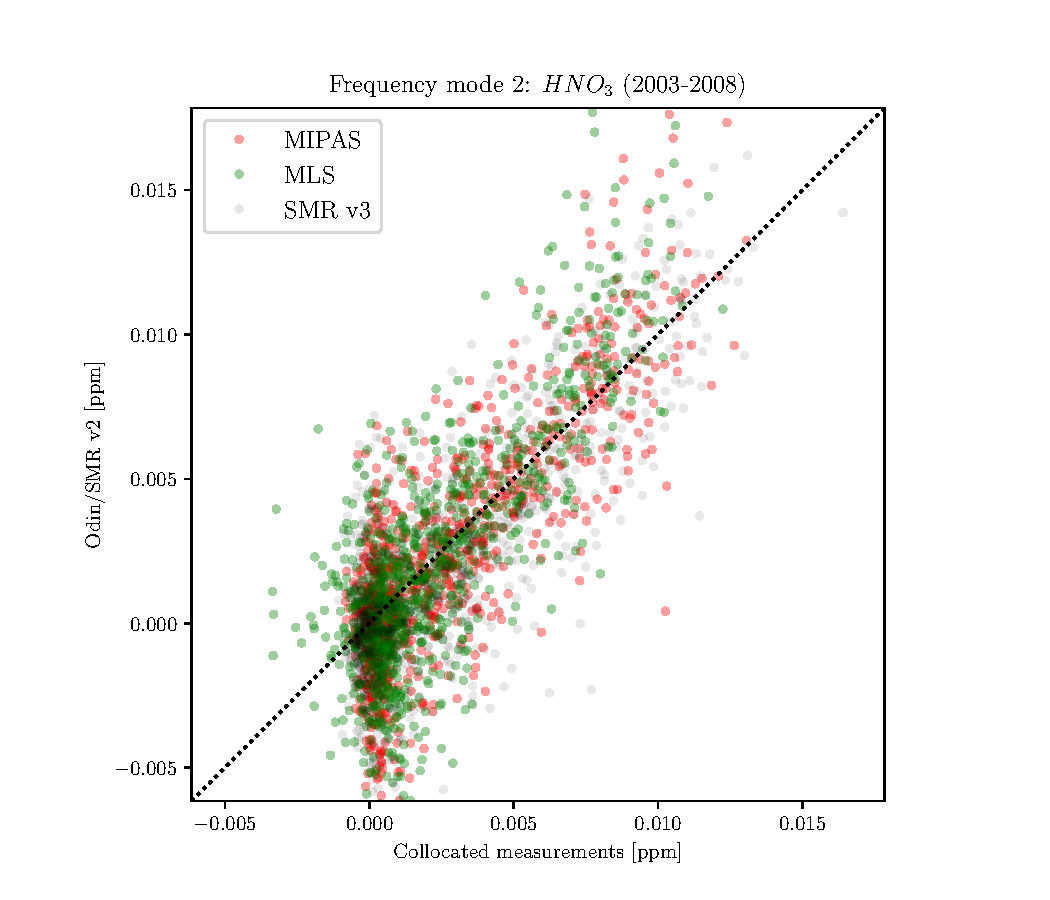
\includegraphics[width=\textwidth]{DDS_fm2_HNO3_scatter_v2}
        \caption{correlation of collcated instruments with \smr~v2.X}
        \label{fig:fm02:HNO3:scatter:v2}
    \end{subfigure}
    \,
    \begin{subfigure}[b]{0.49\textwidth}
        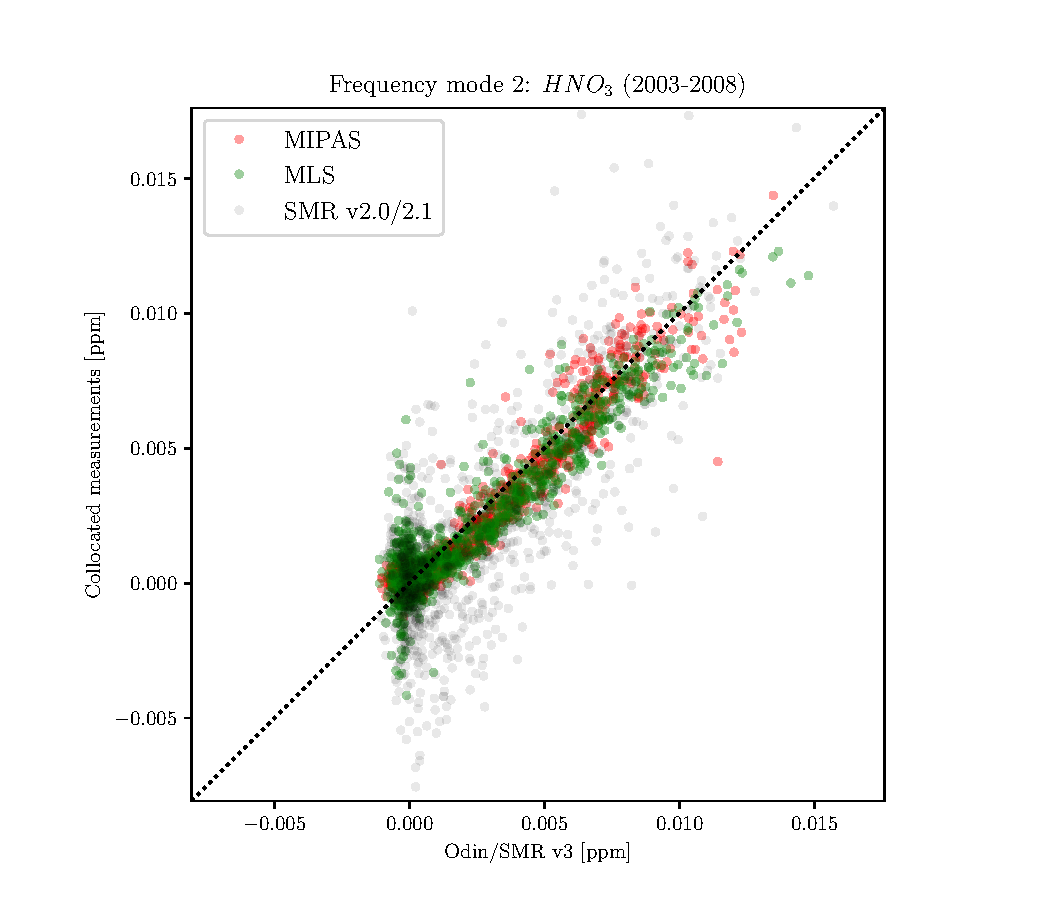
\includegraphics[width=\textwidth]{DDS_fm2_HNO3_scatter_v3}
        \caption{correlation of collcated instruments with \smr~v3}
        \label{fig:fm02:HNO3:scatter:v3}
    \end{subfigure}
    \caption{Correlation between retrievals of \chem{HNO_3} using \smr\
    versions~2.X and~3 and collocated measurements from various instruments.}
    \label{fig:fm02:HNO3:scatter}
\end{figure}

\begin{figure}[htpb]
    \centering
    \begin{subfigure}[b]{0.49\textwidth}
        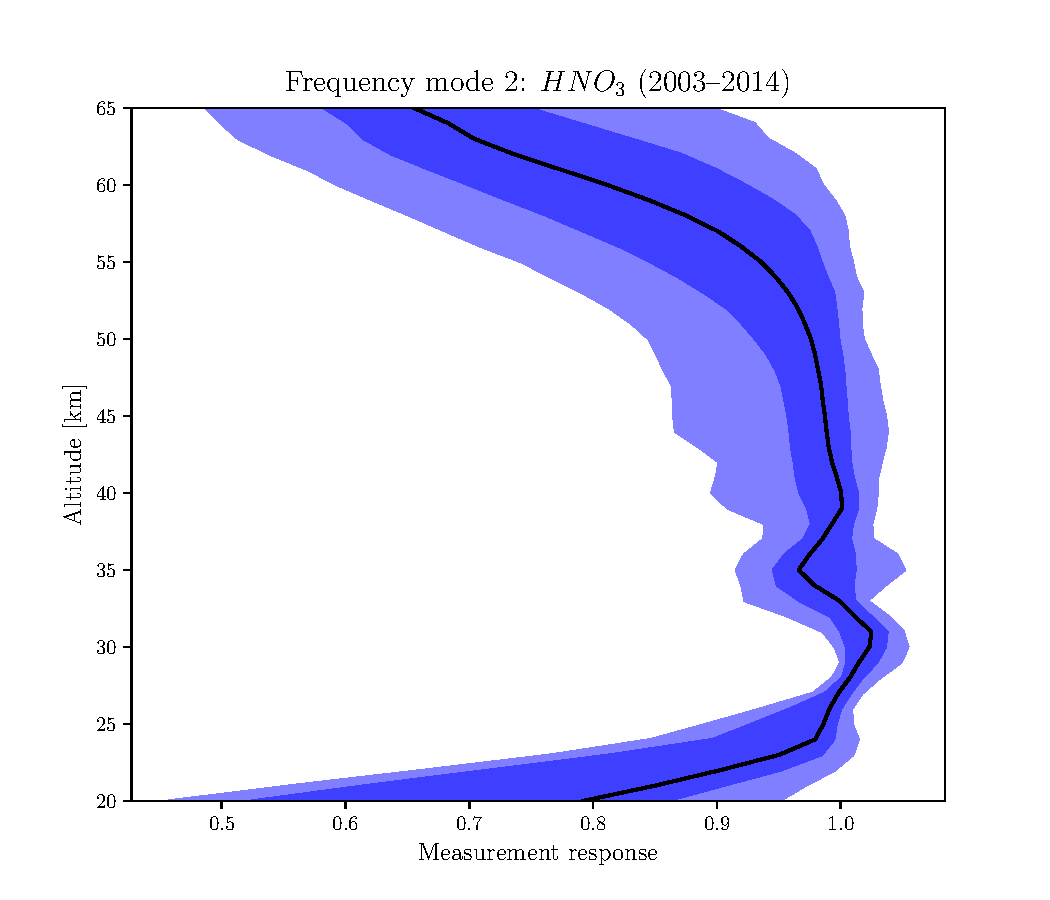
\includegraphics[width=\textwidth]{DDS_fm2_HNO3_mr}
        \caption{median measurement response with $1\sigma$ and $2\sigma$
        percentiles}
        \label{fig:fm02:HNO3:mr}
    \end{subfigure}
    \,
    \begin{subfigure}[b]{0.49\textwidth}
        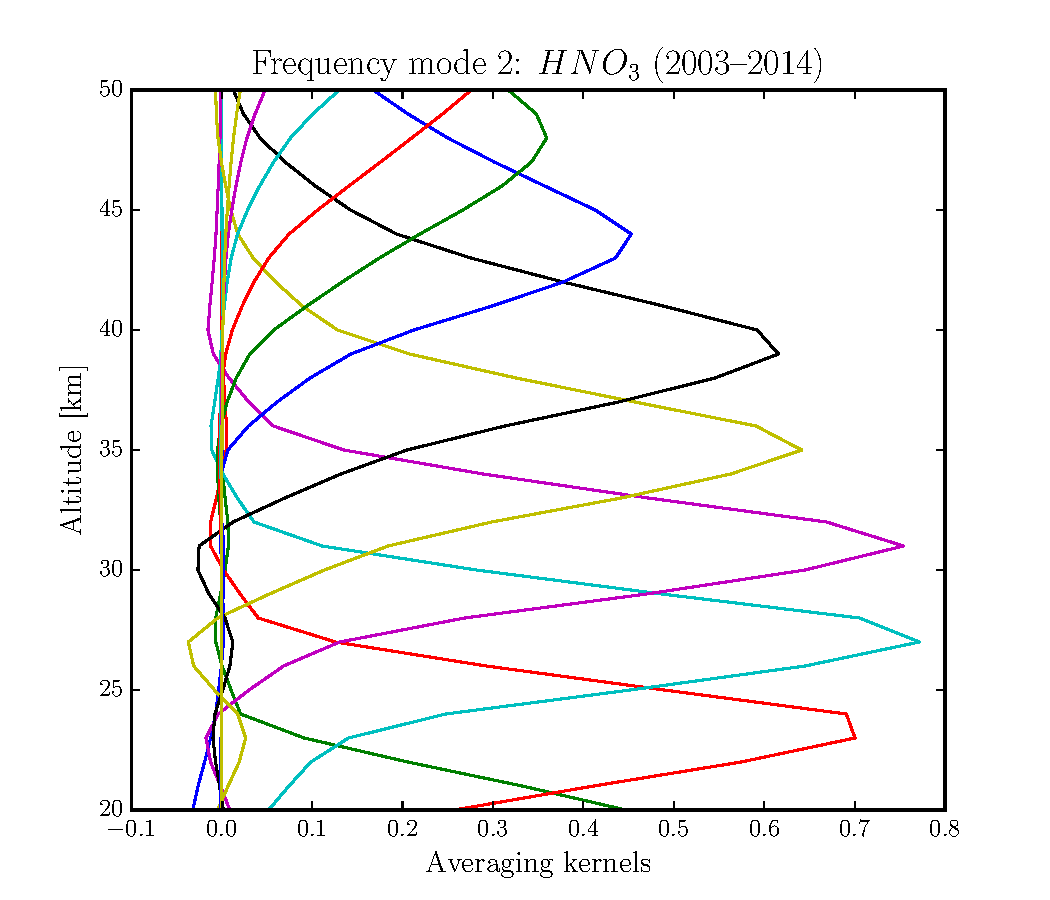
\includegraphics[width=\textwidth]{DDS_fm2_HNO3_avk}
        \caption{median averaging kernels\newline~}
        \label{fig:fm02:HNO3:avk}
    \end{subfigure}
    \caption{Measurement response and averaging kernels for \chem{HNO_3}
    retrievals for \smr~v3 at different altitudes for frequency mode~02.}
    \label{fig:fm02:HNO3:mr_avk}
\end{figure}


%%%%%%%%%%%%%%%
% Temperature %
%%%%%%%%%%%%%%%

\subsubsection{\chem{Temperature}}
\label{sec:fm02:comparison:temperature}
The retrievals for temperature have been compared with data from the MLS
instrument. Annual average differences to this instruments are shown in
Figure~\ref{fig:fm02:T:profiles}. In Figure~\ref{fig:fm02:T:scatter} individual
retrievals from MLS for the entire period are plotted against the
retrievals from the new and old versions of the \smr\ processing chain. The
results show a considerable improvement with the updated version of the
processing, with much better over-all correlation and coherrency, though a
small systematic under estimation of the temperature remains, in particular at
high altitudes.  
Figure~\ref{fig:fm02:T:mr_avk} suggests that the product is useful over the range 10-50 km with a vertical resolution of around 4 km. 

\begin{figure}[htpb]
    \centering
    \begin{subfigure}[b]{0.49\textwidth}
        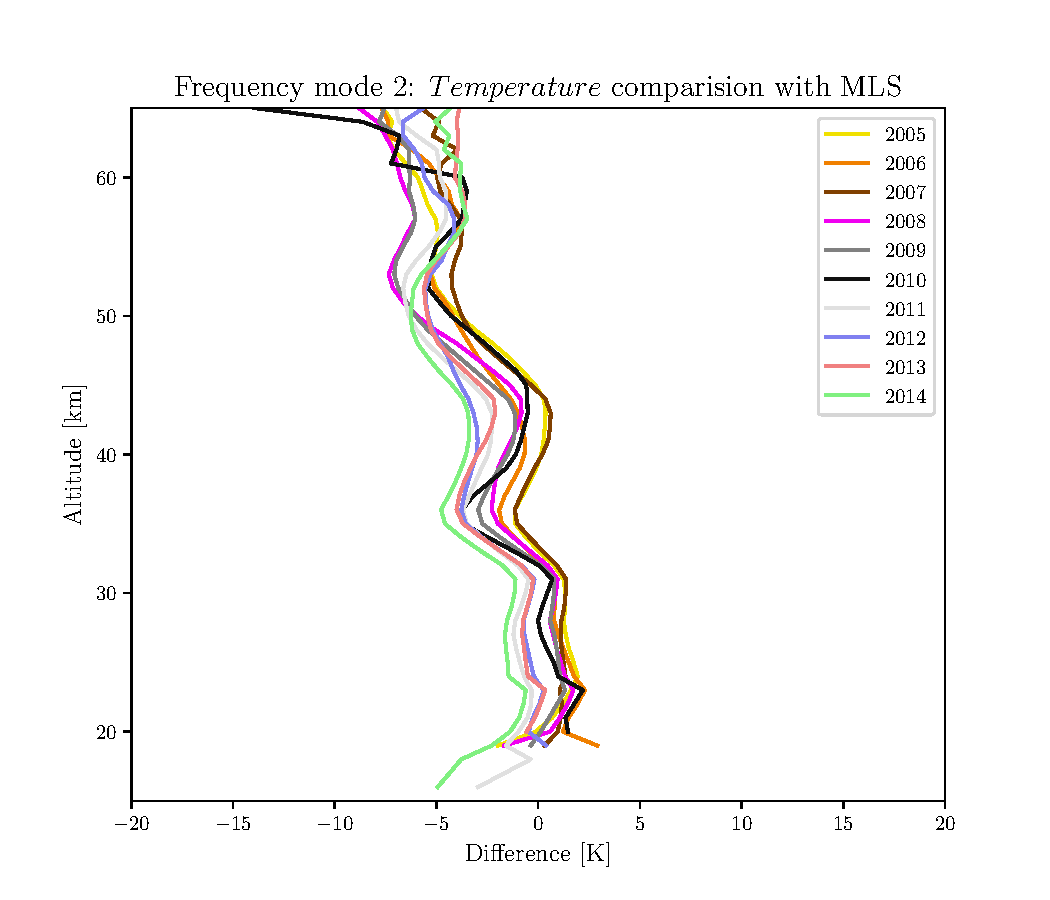
\includegraphics[width=\textwidth]{DDS_fm2_T_absdiff_mls}
        \caption{average difference to MLS}
        \label{fig:fm02:T:profiles:MLS}
    \end{subfigure}
    \caption{Average difference in K between retrievals of temperature from
    \smr~v3 and collocated measurements from MLS at different altitudes.}
    \label{fig:fm02:T:profiles}
\end{figure}

\begin{figure}[htpb]
    \centering
    \begin{subfigure}[b]{0.49\textwidth}
        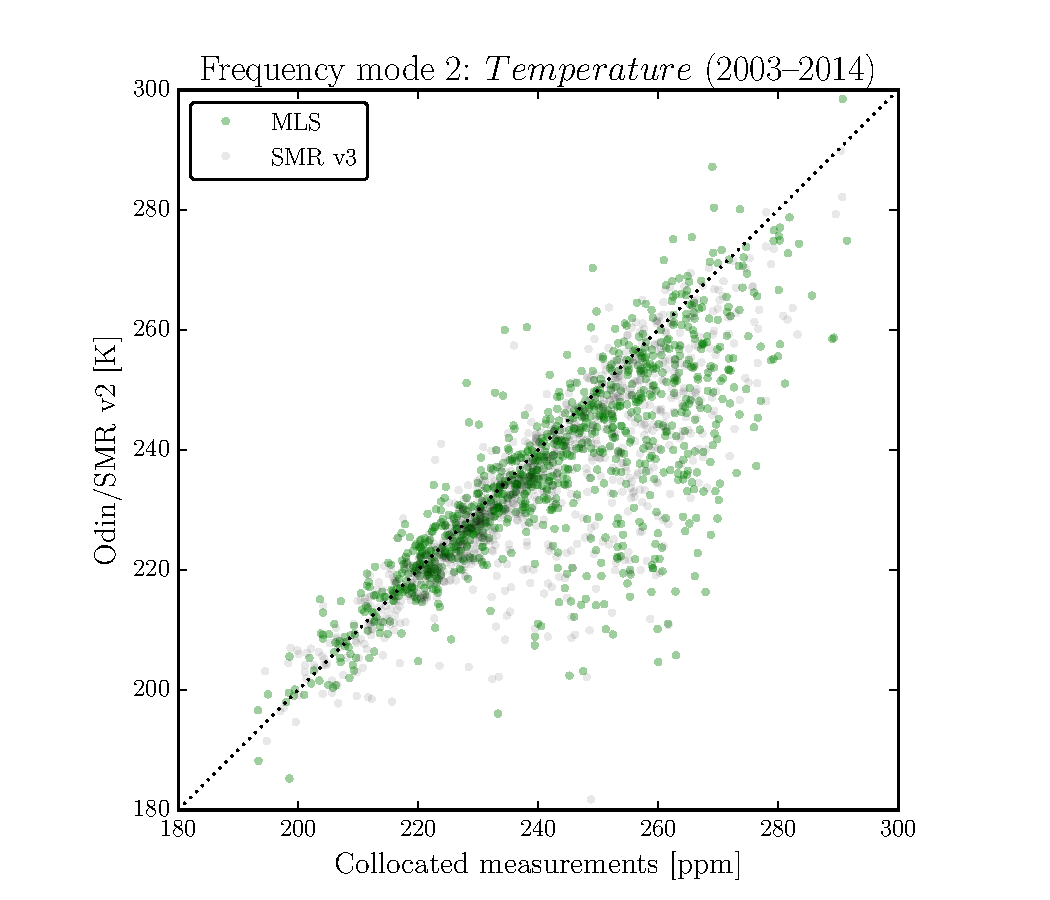
\includegraphics[width=\textwidth]{DDS_fm2_T_scatter_v2}
        \caption{correlation of collcated instruments with \smr~v2.X}
        \label{fig:fm02:T:scatter:v2}
    \end{subfigure}
    \,
    \begin{subfigure}[b]{0.49\textwidth}
        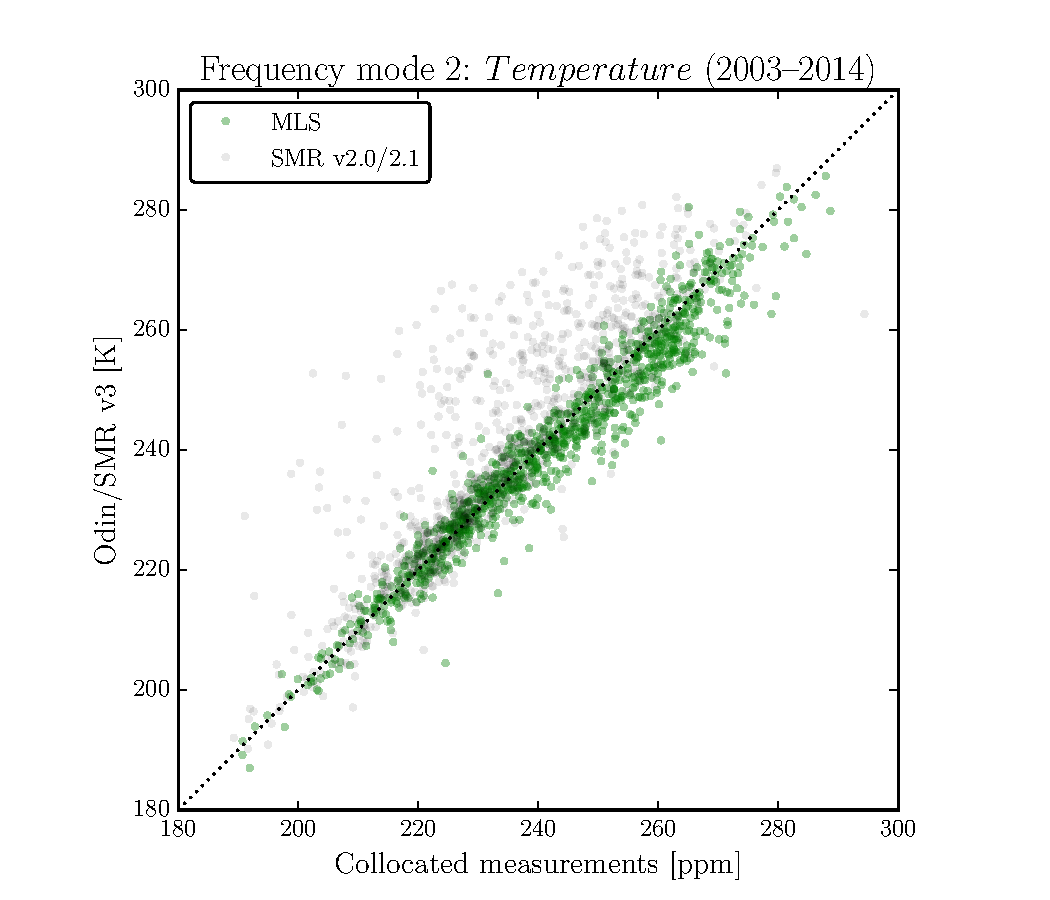
\includegraphics[width=\textwidth]{DDS_fm2_T_scatter_v3}
        \caption{correlation of collcated instruments with \smr~v3}
        \label{fig:fm02:T:scatter:v3}
    \end{subfigure}
    \caption{Correlation between retrievals of temperature using \smr\
    versions~2.X and~3 and collocated measurements from various instruments.}
    \label{fig:fm02:T:scatter}
\end{figure}

\begin{figure}[htpb]
    \centering
    \begin{subfigure}[b]{0.49\textwidth}
        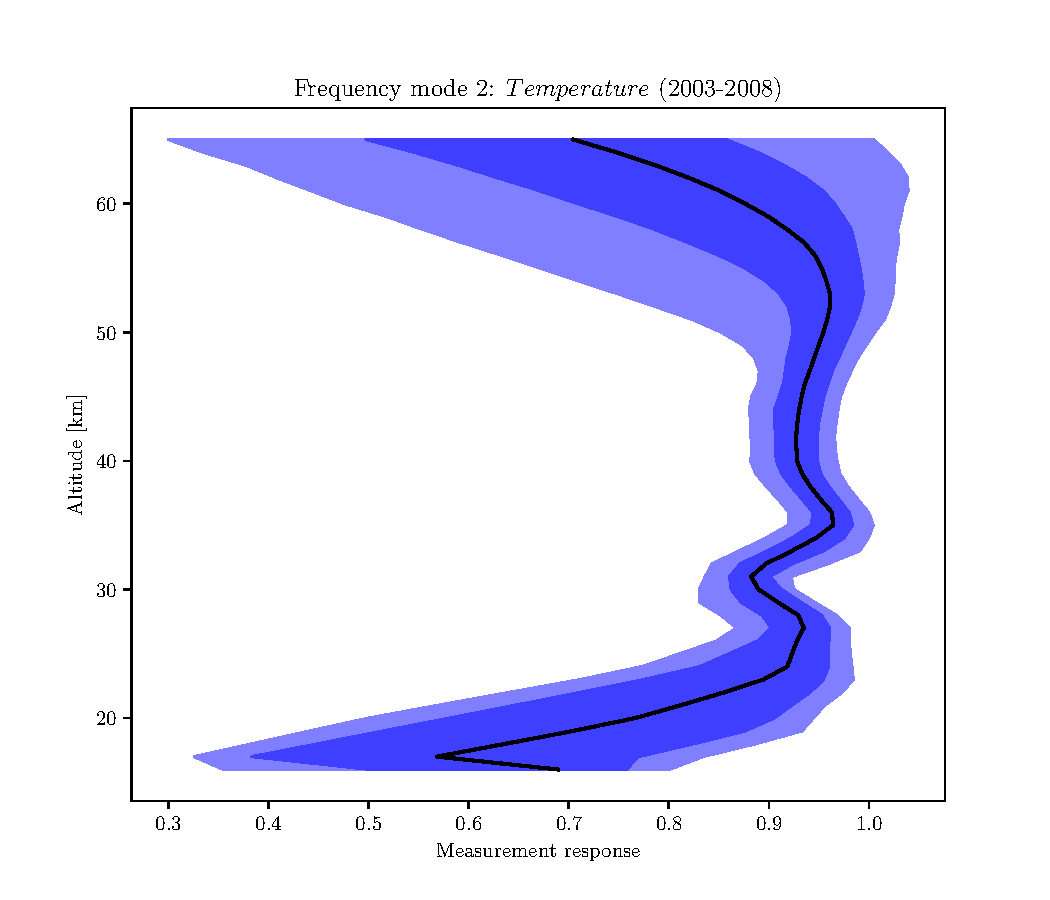
\includegraphics[width=\textwidth]{DDS_fm2_T_mr}
        \caption{median measurement response with $1\sigma$ and $2\sigma$
        percentiles}
        \label{fig:fm02:T:mr}
    \end{subfigure}
    \,
    \begin{subfigure}[b]{0.49\textwidth}
        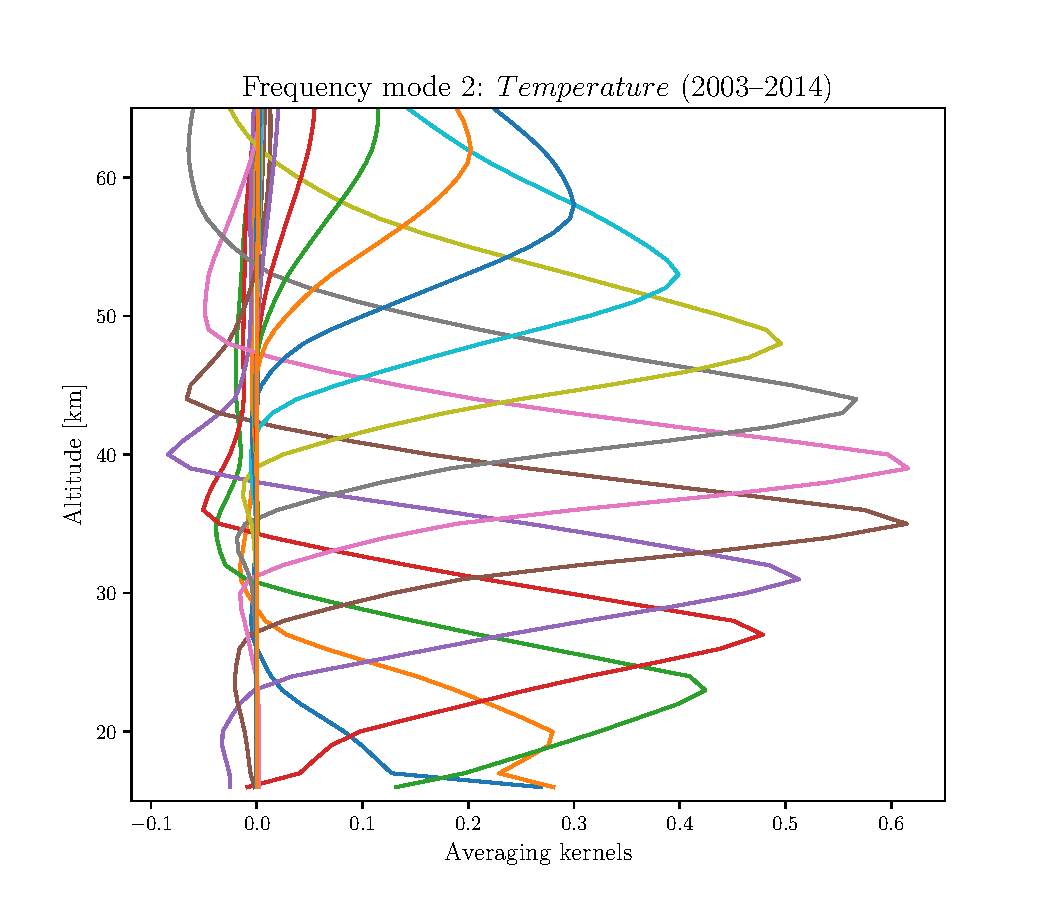
\includegraphics[width=\textwidth]{DDS_fm2_T_avk}
        \caption{median averaging kernels\newline~}
        \label{fig:fm02:T:avk}
    \end{subfigure}
    \caption{Measurement response and averaging kernels for temperature
    retrievals for \smr~v3 at different altitudes for frequency mode~02.}
    \label{fig:fm02:T:mr_avk}
\end{figure}


\subsection{Discussion}
\label{sec:fm02:discussion}
The Pearson correlation between the \smr\ retrievals and the other instruments
was calculated for the entire period for both versions of the processing chain.
The results are summarised in Table~\ref{tab:fm02:stats}, and show that the
new algorithm is a improvement compared to all the instruments for all species
used in this investigation. The improvement is considerable for both \chem{O_3}
and \chem{HNO_3}.


\begin{table}[hbt]
\centering
\caption{Pearson correlation and fit parameters of the old and new \smr\
retrievals for frequency mode~02, compared with collocated data from other
instruments for the period 2003--2014.
}
\label{tab:fm02:stats}
\begin{tabular}{lllrrrr}
    \toprule
    \textbf{Species} & \textbf{Instrument} & \textbf{SMR} & \textbf{corr.} & \textbf{slope} & \textbf{intercept} & \textbf{$\left|\left<\right.\right.$res.$\left.\left.\right>\right|$} \\
    \midrule
    \chem{O3}       & MIPAS     & v3    & 0.966 & 0.925 & -0.070\,ppm   & 0.792\,ppm \\
                    &           & v2.x  & 0.924 & 0.802 & -0.271\,ppm   & 1.449\,ppm \\
    \cline{2-7}
                    & MLS       & v3    & 0.969 & 0.955 & -0.014\,ppm   & 0.681\,ppm \\
                    &           & v2.x  & 0.913 & 0.822 & -0.219\,ppm   & 1.343\,ppm \\
    \cline{2-7}
                    & OSIRIS    & v3    & 0.968 & 0.948 & 0.029\,ppm    & 0.587\,ppm \\
                    &           & v2.x  & 0.918 & 0.812 & -0.187\,ppm   & 1.376\,ppm \\
    \cline{2-7}
                    & SAGE III  & v3    & 0.928 & 1.065 & -0.110\,ppm   & 0.391\,ppm \\
                    &           & v2.x  & 0.742 & 0.795 & -0.152\,ppm   & 0.780\,ppm \\
    \midrule
    \chem{HNO_3}    & MIPAS     & v3    & 0.960 & 0.978 & 0.180\,ppb    & 0.861\,ppb \\
                    &           & v2.x  & 0.819 & 1.049 & -0.395\,ppb    & 2.207\,ppb \\
    \cline{2-7}
                    & MLS       & v3    & 0.924 & 0.976 & 0.280\,ppb    & 1.188\,ppb \\
                    &           & v2.x  & 0.781 & 1.047 & -0.251\,ppb    & 2.442\,ppb \\
    \midrule
    Temp.           & MLS       & v3    & 0.956 & 0.936 & 12.856\,K     &  6.002\,K \\
                    &           & v2.x  & 0.786 & 0.697 & 66.735\,K     & 13.794\,K \\
    \bottomrule
\end{tabular}
\end{table}

\subsection{Conclusions}
\label{sec:fm02:conclusions}

Based on the discussion above, retrievals based on frequency mode~02 can be
used with confidence for the species \chem{O_3} and \chem{HNO_3}, as well as
for temperature.  
